\documentclass[11pt,addpoints,answers]{exam}


%%%%%%%%%%%%%%%%%%%%%%%%%%%%%%%%%%%%%%%%%%%
% Commands for customizing the assignment %
%%%%%%%%%%%%%%%%%%%%%%%%%%%%%%%%%%%%%%%%%%%
\newcommand{\hwNum}{Homework 9}
\newcommand{\hwTopic}{Learning Paradigms}
\newcommand{\hwName}{\hwNum: \hwTopic}
\newcommand{\outDate}{Monday, November 25}
\newcommand{\dueDate}{Thursday, December 5}
\newcommand{\taNames}{Doris, Jenny, Rohan, Siyan, Zoe, Markov, Neural}
\newcommand{\homeworktype}{\string written}

\newcommand{\summary}{
    \begin{notebox}
        \paragraph{Summary} This is the final homework assignment. This assignment covers \textbf{Ensemble Methods}, \textbf{$k$-Means}, \textbf{PCA}, and \textbf{Recommender Systems}.
    \end{notebox}
}

%% To HIDE SOLUTIONS (to post at the website for students), set this value to 0: \def\issoln{0}
\providecommand{\issoln}{1}
% \providecommand{\issoln}{0}

 %-----------------------------------------------------------------------------
% PACKAGES AND OTHER DOCUMENT CONFIGURATIONS
%-----------------------------------------------------------------------------

\usepackage[margin=1in]{geometry}
\usepackage{bbm}
\usepackage{amsmath, amsfonts}
\usepackage{enumerate}
\usepackage{graphicx}
\usepackage{titling}
\usepackage{url}
\usepackage{xfrac}
\usepackage{natbib}
\usepackage{amssymb}
\usepackage{amsthm}
\usepackage{paralist}
\usepackage{epstopdf}
\usepackage{tabularx}
\usepackage{longtable}
\usepackage{multirow}
\usepackage{multicol}
\usepackage[colorlinks=true,urlcolor=blue]{hyperref}
\usepackage{algorithm}
\usepackage{algorithmicx}
\usepackage[noend]{algpseudocode}
\usepackage{float}
\usepackage{enumerate}
\usepackage{array}
\usepackage{environ}
\usepackage{times}
\usepackage{textcomp}
\usepackage{caption}
\usepackage{parskip} % For NIPS style paragraphs.
\usepackage[compact]{titlesec} % Less whitespace around titles
\usepackage[inline]{enumitem} % For inline enumerate* and itemize*
\usepackage{datetime}
\usepackage{comment}
% \usepackage{minted}
\usepackage{lastpage}
\usepackage{color}
\usepackage{xcolor}
\usepackage[final]{listings}
\usepackage{framed}
\usepackage{booktabs}
\usepackage{cprotect}
\usepackage{verbatim}
\usepackage{verbatimbox}
\usepackage{multicol}
\usepackage{hyperref}
\usepackage{subcaption}
\usepackage{mathtools} % For drcases
\usepackage{cancel}
\usepackage[many]{tcolorbox}
\usepackage{soul}
\usepackage[bottom]{footmisc}
\usepackage{bm}
\usepackage{wasysym}
\usepackage{pgfplots}
\usepackage{tikz}
\usetikzlibrary{shapes,decorations,arrows}
\usetikzlibrary{arrows.meta}
\usetikzlibrary{shapes.geometric}
\usetikzlibrary{positioning, arrows, automata, calc}
\usepackage{transparent}
\usepackage{tikz-cd}


\newtcolorbox[]{your_solution}[1][]{
    % breakable,
    enhanced,
    nobeforeafter,
    colback=white,
    title=Your Answer,
    sidebyside align=top,
    box align=top,
    #1
}


%%%%%%%%%%%%%%%%%%%%%%%%%%%%%%%%%%%%%%%%%%%
% Rotated Column Headers                  %
%%%%%%%%%%%%%%%%%%%%%%%%%%%%%%%%%%%%%%%%%%%
\usepackage{adjustbox}
\usepackage{array}

%https://tex.stackexchange.com/questions/32683/rotated-column-titles-in-tabular

\newcolumntype{R}[2]{%
    >{\adjustbox{angle=#1,lap=\width-(#2)}\bgroup}%
    l%
    <{\egroup}%
}
\newcommand*\rot{\multicolumn{1}{R{45}{1em}}}% no optional argument here, please!


%%%%%%%%%%%%%%%%%%%%%%%%%%%%%%%%%%%%%%%%%%%
% Formatting for \CorrectChoice of "exam" %
%%%%%%%%%%%%%%%%%%%%%%%%%%%%%%%%%%%%%%%%%%%

\CorrectChoiceEmphasis{}
\checkedchar{\blackcircle}

\newenvironment{checkboxessquare}{
    \begingroup
    \checkboxchar{$\Box$} \checkedchar{$\blacksquare$} % change checkbox style locally
    \begin{checkboxes}
    }{
    \end{checkboxes}
    \endgroup
    }

%%%%%%%%%%%%%%%%%%%%%%%%%%%%%%%%%%%%%%%%%%%
% Better numbering                        %
%%%%%%%%%%%%%%%%%%%%%%%%%%%%%%%%%%%%%%%%%%%

% \numberwithin{equation}{section} % Number equations within sections (i.e. 1.1, 1.2, 2.1, 2.2 instead of 1, 2, 3, 4)
% \numberwithin{figure}{section} % Number figures within sections (i.e. 1.1, 1.2, 2.1, 2.2 instead of 1, 2, 3, 4)
% \numberwithin{table}{section} % Number tables within sections (i.e. 1.1, 1.2, 2.1, 2.2 instead of 1, 2, 3, 4)

%%%%%%%%%%%%%%%%%%%%%%%%%%%%%%%%%%%%%%%%%%
% Custom commands                        %
%%%%%%%%%%%%%%%%%%%%%%%%%%%%%%%%%%%%%%%%%%
\newcommand{\R}{\mathbb{R}}
\newcommand{\blackcircle}{\tikz\draw[black,fill=black] (0,0) circle (1ex);}
\renewcommand{\circle}{\tikz\draw[black] (0,0) circle (1ex);}


%%%%%%%%%%%%%%%%%%%%%%%%%%%%%%%%%%%%%%%%%%
% Custom commands for Math               %
%%%%%%%%%%%%%%%%%%%%%%%%%%%%%%%%%%%%%%%%%%
\newcommand{\vc}[1]{\boldsymbol{#1}}
\newcommand{\adj}[1]{\frac{\partial \ell}{\partial #1}}
\newcommand{\chain}[2]{\adj{#2} = \adj{#1}\frac{\partial #1}{\partial #2}}
\newcommand{\ntset}{test}
\newcommand{\zerov}{\mathbf{0}}
\DeclareMathOperator*{\argmin}{argmin}

% mathcal
\newcommand{\Ac}{\mathcal{A}}
\newcommand{\Bc}{\mathcal{B}}
\newcommand{\Cc}{\mathcal{C}}
\newcommand{\Dc}{\mathcal{D}}
\newcommand{\Ec}{\mathcal{E}}
\newcommand{\Fc}{\mathcal{F}}
\newcommand{\Gc}{\mathcal{G}}
\newcommand{\Hc}{\mathcal{H}}
\newcommand{\Ic}{\mathcal{I}}
\newcommand{\Jc}{\mathcal{J}}
\newcommand{\Kc}{\mathcal{K}}
\newcommand{\Lc}{\mathcal{L}}
\newcommand{\Mc}{\mathcal{M}}
\newcommand{\Nc}{\mathcal{N}}
\newcommand{\Oc}{\mathcal{O}}
\newcommand{\Pc}{\mathcal{P}}
\newcommand{\Qc}{\mathcal{Q}}
\newcommand{\Rc}{\mathcal{R}}
\newcommand{\Sc}{\mathcal{S}}
\newcommand{\Tc}{\mathcal{T}}
\newcommand{\Uc}{\mathcal{U}}
\newcommand{\Vc}{\mathcal{V}}
\newcommand{\Wc}{\mathcal{W}}
\newcommand{\Xc}{\mathcal{X}}
\newcommand{\Yc}{\mathcal{Y}}
\newcommand{\Zc}{\mathcal{Z}}

% mathbb
\newcommand{\Ab}{\mathbb{A}}
\newcommand{\Bb}{\mathbb{B}}
\newcommand{\Cb}{\mathbb{C}}
\newcommand{\Db}{\mathbb{D}}
\newcommand{\Eb}{\mathbb{E}}
\newcommand{\Fb}{\mathbb{F}}
\newcommand{\Gb}{\mathbb{G}}
\newcommand{\Hb}{\mathbb{H}}
\newcommand{\Ib}{\mathbb{I}}
\newcommand{\Jb}{\mathbb{J}}
\newcommand{\Kb}{\mathbb{K}}
\newcommand{\Lb}{\mathbb{L}}
\newcommand{\Mb}{\mathbb{M}}
\newcommand{\Nb}{\mathbb{N}}
\newcommand{\Ob}{\mathbb{O}}
\newcommand{\Pb}{\mathbb{P}}
\newcommand{\Qb}{\mathbb{Q}}
\newcommand{\Rb}{\mathbb{R}}
\newcommand{\Sb}{\mathbb{S}}
\newcommand{\Tb}{\mathbb{T}}
\newcommand{\Ub}{\mathbb{U}}
\newcommand{\Vb}{\mathbb{V}}
\newcommand{\Wb}{\mathbb{W}}
\newcommand{\Xb}{\mathbb{X}}
\newcommand{\Yb}{\mathbb{Y}}
\newcommand{\Zb}{\mathbb{Z}}

% mathbf lowercase
\newcommand{\av}{\mathbf{a}}
\newcommand{\bv}{\mathbf{b}}
\newcommand{\cv}{\mathbf{c}}
\newcommand{\dv}{\mathbf{d}}
\newcommand{\ev}{\mathbf{e}}
\newcommand{\fv}{\mathbf{f}}
\newcommand{\gv}{\mathbf{g}}
\newcommand{\hv}{\mathbf{h}}
\newcommand{\iv}{\mathbf{i}}
\newcommand{\jv}{\mathbf{j}}
\newcommand{\kv}{\mathbf{k}}
\newcommand{\lv}{\mathbf{l}}
\newcommand{\mv}{\mathbf{m}}
\newcommand{\nv}{\mathbf{n}}
\newcommand{\ov}{\mathbf{o}}
\newcommand{\pv}{\mathbf{p}}
\newcommand{\qv}{\mathbf{q}}
\newcommand{\rv}{\mathbf{r}}
\newcommand{\sv}{\mathbf{s}}
\newcommand{\tv}{\mathbf{t}}
\newcommand{\uv}{\mathbf{u}}
\newcommand{\vv}{\mathbf{v}}
\newcommand{\wv}{\mathbf{w}}
\newcommand{\xv}{\mathbf{x}}
\newcommand{\yv}{\mathbf{y}}
\newcommand{\zv}{\mathbf{z}}

% mathbf uppercase
\newcommand{\Av}{\mathbf{A}}
\newcommand{\Bv}{\mathbf{B}}
\newcommand{\Cv}{\mathbf{C}}
\newcommand{\Dv}{\mathbf{D}}
\newcommand{\Ev}{\mathbf{E}}
\newcommand{\Fv}{\mathbf{F}}
\newcommand{\Gv}{\mathbf{G}}
\newcommand{\Hv}{\mathbf{H}}
\newcommand{\Iv}{\mathbf{I}}
\newcommand{\Jv}{\mathbf{J}}
\newcommand{\Kv}{\mathbf{K}}
\newcommand{\Lv}{\mathbf{L}}
\newcommand{\Mv}{\mathbf{M}}
\newcommand{\Nv}{\mathbf{N}}
\newcommand{\Ov}{\mathbf{O}}
\newcommand{\Pv}{\mathbf{P}}
\newcommand{\Qv}{\mathbf{Q}}
\newcommand{\Rv}{\mathbf{R}}
\newcommand{\Sv}{\mathbf{S}}
\newcommand{\Tv}{\mathbf{T}}
\newcommand{\Uv}{\mathbf{U}}
\newcommand{\Vv}{\mathbf{V}}
\newcommand{\Wv}{\mathbf{W}}
\newcommand{\Xv}{\mathbf{X}}
\newcommand{\Yv}{\mathbf{Y}}
\newcommand{\Zv}{\mathbf{Z}}

% bold greek lowercase
\newcommand{\alphav     }{\boldsymbol \alpha     }
\newcommand{\betav      }{\boldsymbol \beta      }
\newcommand{\gammav     }{\boldsymbol \gamma     }
\newcommand{\deltav     }{\boldsymbol \delta     }
\newcommand{\epsilonv   }{\boldsymbol \epsilon   }
\newcommand{\varepsilonv}{\boldsymbol \varepsilon}
\newcommand{\zetav      }{\boldsymbol \zeta      }
\newcommand{\etav       }{\boldsymbol \eta       }
\newcommand{\thetav     }{\boldsymbol \theta     }
\newcommand{\varthetav  }{\boldsymbol \vartheta  }
\newcommand{\iotav      }{\boldsymbol \iota      }
\newcommand{\kappav     }{\boldsymbol \kappa     }
\newcommand{\varkappav  }{\boldsymbol \varkappa  }
\newcommand{\lambdav    }{\boldsymbol \lambda    }
\newcommand{\muv        }{\boldsymbol \mu        }
\newcommand{\nuv        }{\boldsymbol \nu        }
\newcommand{\xiv        }{\boldsymbol \xi        }
\newcommand{\omicronv   }{\boldsymbol \omicron   }
\newcommand{\piv        }{\boldsymbol \pi        }
\newcommand{\varpiv     }{\boldsymbol \varpi     }
\newcommand{\rhov       }{\boldsymbol \rho       }
\newcommand{\varrhov    }{\boldsymbol \varrho    }
\newcommand{\sigmav     }{\boldsymbol \sigma     }
\newcommand{\varsigmav  }{\boldsymbol \varsigma  }
\newcommand{\tauv       }{\boldsymbol \tau       }
\newcommand{\upsilonv   }{\boldsymbol \upsilon   }
\newcommand{\phiv       }{\boldsymbol \phi       }
\newcommand{\varphiv    }{\boldsymbol \varphi    }
\newcommand{\chiv       }{\boldsymbol \chi       }
\newcommand{\psiv       }{\boldsymbol \psi       }
\newcommand{\omegav     }{\boldsymbol \omega     }

% bold greek uppercase
\newcommand{\Gammav     }{\boldsymbol \Gamma     }
\newcommand{\Deltav     }{\boldsymbol \Delta     }
\newcommand{\Thetav     }{\boldsymbol \Theta     }
\newcommand{\Lambdav    }{\boldsymbol \Lambda    }
\newcommand{\Xiv        }{\boldsymbol \Xi        }
\newcommand{\Piv        }{\boldsymbol \Pi        }
\newcommand{\Sigmav     }{\boldsymbol \Sigma     }
\newcommand{\Upsilonv   }{\boldsymbol \Upsilon   }
\newcommand{\Phiv       }{\boldsymbol \Phi       }
\newcommand{\Psiv       }{\boldsymbol \Psi       }
\newcommand{\Omegav     }{\boldsymbol \Omega     }

%%%%%%%%%%%%%%%%%%%%%%%%%%%%%%%%%%%%%%%%%%%
% Code highlighting with listings         %
%%%%%%%%%%%%%%%%%%%%%%%%%%%%%%%%%%%%%%%%%%%

\definecolor{bluekeywords}{rgb}{0.13,0.13,1}
\definecolor{greencomments}{rgb}{0,0.5,0}
\definecolor{redstrings}{rgb}{0.9,0,0}
\definecolor{light-gray}{gray}{0.95}

\newcommand{\MYhref}[3][blue]{\href{#2}{\color{#1}{#3}}}%

\definecolor{dkgreen}{rgb}{0,0.6,0}
\definecolor{gray}{rgb}{0.5,0.5,0.5}
\definecolor{mauve}{rgb}{0.58,0,0.82}

\lstdefinelanguage{Shell}{
  keywords={tar, cd, make},
  %keywordstyle=\color{bluekeywords}\bfseries,
  alsoletter={+},
  ndkeywords={python, py, javac, java, gcc, c, g++, cpp, .txt, octave, m, .tar},
  %ndkeywordstyle=\color{bluekeywords}\bfseries,
  identifierstyle=\color{black},
  sensitive=false,
  comment=[l]{//},
  morecomment=[s]{/*}{*/},
  commentstyle=\color{purple}\ttfamily,
  %stringstyle=\color{red}\ttfamily,
  morestring=[b]',
  morestring=[b]",
  backgroundcolor = \color{light-gray}
}

\lstset{columns=fixed, basicstyle=\ttfamily,
    backgroundcolor=\color{light-gray},xleftmargin=0.5cm,frame=tlbr,framesep=4pt,framerule=0pt}

\newcommand{\emptysquare}{{\LARGE $\square$}\ \ }
\newcommand{\filledsquare}{{\LARGE $\boxtimes$}\ \ }
\def \ifempty#1{\def\temp{#1} \ifx\temp\empty }

\def \squaresolutionspace#1{ \ifempty{#1} \emptysquare \else #1\hspace{0.75pt}\fi}

\newcommand{\emptycircle}{{\LARGE $\fullmoon$}\ \ }
\newcommand{\filledcircle}{{\LARGE $\newmoon$}\ \ }
\def \circlesolutionspace#1{ \ifempty{#1} \emptycircle \else #1\hspace{0.75pt}\fi}

%%%%%%%%%%%%%%%%%%%%%%%%%%%%%%%%%%%%%%%%%%%
% Custom box for highlights               %
%%%%%%%%%%%%%%%%%%%%%%%%%%%%%%%%%%%%%%%%%%%

% Define box and box title style
\tikzstyle{mybox} = [fill=blue!10, very thick,
    rectangle, rounded corners, inner sep=1em, inner ysep=1em]

% \newcommand{\notebox}[1]{
% \begin{tikzpicture}
% \node [mybox] (box){%
%     \begin{minipage}{\textwidth}
%     #1
%     \end{minipage}
% };
% \end{tikzpicture}%
% }

\NewEnviron{notebox}{

\begin{tikzpicture}
\node [mybox] (box){
    \begin{minipage}{\textwidth}
        \BODY
    \end{minipage}
};
\end{tikzpicture}
}

%%%%%%%%%%%%%%%%%%%%%%%%%%%%%%%%%%%%%%%%%%%
% Commands showing / hiding solutions     %
%%%%%%%%%%%%%%%%%%%%%%%%%%%%%%%%%%%%%%%%%%%

%%%%%%%%%%%%%%%%%%%%%%%%%%%%%%%%%%%%%%%%%%%
% Commands showing / hiding solutions     %
%%%%%%%%%%%%%%%%%%%%%%%%%%%%%%%%%%%%%%%%%%%
\newcommand{\solutionspace}[4]{\fbox{\begin{minipage}[t][#1][t]{#2} \textbf{#3} \solution{}{#4} \end{minipage}}}

%% To HIDE SOLUTIONS (to post at the website for students), set this value to 0: \def\issoln{0}
% \def\issoln{0} % Uncomment to remove solutions
% \def\issoln{1} % Uncomment to show solutions

% Some commands to allow solutions to be embedded in the assignment file.
\ifcsname issoln\endcsname \else \def\issoln{1} \fi

% Default to an empty solutions environ.
\NewEnviron{soln}{}{}
\if\issoln 1

% Otherwise, include solutions as below.
 \RenewEnviron{soln}{
    \leavevmode\color{red}\ignorespaces   %textbf{Solution} \BODY
    \BODY
 }{}
\fi

%%%%%%%%%%%%%%%%

%% qauthor environment:
% Default to an empty qauthor environ.
\NewEnviron{qauthor}{}{}

%% To HIDE TAGS set this value to 0:
\def\showtags{0}  % Uncomment to remove tags
% \def\showtags{1} % Uncomment to show tags


\ifcsname showtags\endcsname \else \def\showtags{1} \fi

% Default to an empty tags environ.
\NewEnviron{tags}{}{}
\if\showtags 1

% Otherwise, include solutions as below.
\RenewEnviron{tags}{
    \fbox{
    \leavevmode\color{blue}\ignorespaces
    \textbf{TAGS:} \texttt{\url{\BODY}}
    }
    \vspace{-.5em}
}{}
\fi

% Default to an empty learning objective environment
\NewEnviron{qlearningobjective}{}
%%%%%%%%%%%%%%%%%%%%%%%%%%%%%%%%%%%%%%%%%%%%%%%%%
% Useful commands for typesetting the questions %
%%%%%%%%%%%%%%%%%%%%%%%%%%%%%%%%%%%%%%%%%%%%%%%%%

\newcommand \expect {\mathbb{E}}
\newcommand \mle [1]{{\hat #1}^{\rm MLE}}
\newcommand \map [1]{{\hat #1}^{\rm MAP}}
\newcommand \argmax {\operatorname*{argmax}}
% \newcommand \argmin {\operatorname*{argmin}}
\newcommand \code [1]{{\tt #1}}
\newcommand \datacount [1]{\#\{#1\}}
\newcommand \ind [1]{\mathbb{I}\{#1\}}

%%%%%%%%%%%%%%%%%%%%%%%%%%
% Document configuration %
%%%%%%%%%%%%%%%%%%%%%%%%%%

% Don't display a date in the title and remove the white space
\predate{}
\postdate{}
\date{}

% Don't display an author and remove the white space
%\preauthor{}
%\postauthor{}

% Solo and group questions
\newcommand{\solo}{\textbf{[SOLO]} }
\newcommand{\group}{\textbf{[GROUP]} }

% Question type commands
\newcommand{\sall}{\textbf{Select all that apply: }}
\newcommand{\sone}{\textbf{Select one: }}
\newcommand{\tf}{\textbf{True or False: }}

% AdaBoost commands
\newcommand{\trainerr}[1]{\hat{\epsilon}_S \left(#1\right)}
\newcommand{\generr}[1]{\epsilon \left(#1\right)}
\newcommand{\D}{\mathcal{D}}
\newcommand{\margin}{\text{margin}}
\newcommand{\sign}{\text{sign}}
\newcommand{\PrS}{\hat{\Pr_{(x_i, y_i) \sim S}}}
\newcommand{\PrSinline}{\hat{\Pr}_{(x_i, y_i) \sim S}}  % inline PrS

% Abhi messing around with examdoc
\qformat{\textbf{{\Large \thequestion \; \; \thequestiontitle \ (\totalpoints \ points)}} \hfill}
\renewcommand{\thequestion}{\arabic{question}}
\renewcommand{\questionlabel}{\thequestion.}

\renewcommand{\thepartno}{\arabic{partno}}
\renewcommand{\partlabel}{\thepartno.}
\renewcommand{\partshook}{\setlength{\leftmargin}{0pt}}

\renewcommand{\thesubpart}{\alph{subpart}}
\renewcommand{\subpartlabel}{(\thesubpart)}

\renewcommand{\thesubsubpart}{\roman{subsubpart}}
\renewcommand{\subsubpartlabel}{\thesubsubpart.}

% copied from stack overflow, as all good things are
\newcommand\invisiblesection[1]{%
  \refstepcounter{section}%
  \addcontentsline{toc}{section}{\protect\numberline{\thesection}#1}%
  \sectionmark{#1}}

% quite possibly the worst workaround i have made for this class
\newcommand{\sectionquestion}[1]{
\titledquestion{#1}
\invisiblesection{#1}
~\vspace{-1em}
}

% also copied from stack overflow
% https://tex.stackexchange.com/questions/153846/indent-every-subsubsection-element
% and edited following
% https://latexref.xyz/bs-at-startsection.html
% PLEASE DELETE THIS FOR OTHER HOMEWORK
% \ifnum\pdfstrcmp{\taNames}{Sana, Chu, Hayden, Tori, Prasoon}=0
% \makeatletter
% \newcommand\subsectionquestion{%
%   \@startsection{subsection}{2}
%   {-2pc}% <------- The opposite of what we set for subs
%   {-3.25ex\@plus -1ex \@minus -.2ex}%
%   {1.5ex \@plus .2ex}%
%   {\normalfont\large\bfseries}}
% \makeatother
% \fi

%%%%%%%%%%%%%%%%%%%%%%%%%%%%%%%%%%%%%%%%%%%
% New Environment for Pseudocode          %
%%%%%%%%%%%%%%%%%%%%%%%%%%%%%%%%%%%%%%%%%%%

% Python style for highlighting
\DeclareFixedFont{\ttb}{T1}{txtt}{bx}{n}{12} % for bold
\DeclareFixedFont{\ttm}{T1}{txtt}{m}{n}{12}  % for normal

\definecolor{deepblue}{rgb}{0,0,0.5}
\definecolor{deepred}{rgb}{0.6,0,0}
\definecolor{deepgreen}{rgb}{0,0.5,0}

\newcommand\pythonstyle{\lstset{
language=Python,
basicstyle=\ttm,
morekeywords={self},              % Add keywords here
keywordstyle=\ttb\color{deepblue},
emph={MyClass,__init__},          % Custom highlighting
emphstyle=\ttb\color{deepred},    % Custom highlighting style
stringstyle=\color{deepgreen},
frame=tb,                         % Any extra options here
showstringspaces=false
}}


% Python environment
\lstnewenvironment{your_code_solution}[1][]
{
\pythonstyle
\lstset{#1}
}
{}
\newtcolorbox[]{your_code_solution_outer}[1][]{
    % breakable,
    enhanced,
    nobeforeafter,
    colback=white,
    title=Your Answer,
    sidebyside align=top,
    box align=top,
    #1
}
%%%%%%%%%%%%%%%%%%%%%%%%%%%%%%%%%%%%%%%%%%%
% Commands for customizing the assignment %
%%%%%%%%%%%%%%%%%%%%%%%%%%%%%%%%%%%%%%%%%%%
\newcommand{\courseNum}{10-301 / 10-601}
\newcommand{\courseName}{Introduction to Machine Learning}
\newcommand{\courseSem}{Fall 2024}
\newcommand{\courseUrl}{\url{http://www.cs.cmu.edu/~mgormley/courses/10601/}}

%\pagestyle{fancyplain}
\lhead{\hwName}
\rhead{\courseNum}
\cfoot{\thepage{} of \numpages{}}

\title{\textsc{\hwNum}: \textsc{\hwTopic} 
\thanks{Compiled on \today{} at \currenttime{}} \\
\vspace{1em}
} % Title

\author{\textsc{\large \courseNum{} \courseName{} (\courseSem)}\\
\courseUrl
\vspace{1em}\\
  OUT: \outDate \\
  DUE: \dueDate \\
  TAs: \taNames\\
}

\date{}
\begin{document}
    \maketitle
    \summary{}
    
\section*{START HERE: Instructions}
\begin{itemize}
\newcommand \maxsubs {10 }

\item \textbf{Collaboration Policy}: Please read the collaboration policy here: \url{http://www.cs.cmu.edu/~mgormley/courses/10601/syllabus.html}

\item\textbf{Late Submission Policy:} See the late submission policy here: \url{http://www.cs.cmu.edu/~mgormley/courses/10601/syllabus.html}

\item\textbf{Submitting your work:} You will use Gradescope to submit
  answers to all questions\ifthenelse{\equal{\homeworktype}{\string written}}{}{ and code}. Please
  follow instructions at the end of this PDF to correctly submit all your code to Gradescope.

\begin{itemize}
    
    \item \textbf{Written:} For written problems such as short answer, multiple choice, derivations, proofs, or plots, please use the provided template. Submissions can be handwritten onto the template, but should be labeled and clearly legible. If your writing is not legible, you will not be awarded marks. Alternatively, submissions can be written in \LaTeX{}. Each derivation/proof should be completed in the boxes provided. You are responsible for ensuring that your submission contains exactly the same number of pages and the same alignment as our PDF template. If you do not follow the template, your assignment may not be graded correctly by our AI assisted grader and there will be a \textbf{\textcolor{red}{2\% penalty}} (e.g., if the homework is out of 100 points, 2 points will be deducted from your final score).
    %
    % This policy is NOT in effect when we have the Background Test.
    % \ifthenelse{\equal{\homeworktype}{\string hw1}}{ {\color{red} For this assignment only, if you answer at least 90\% of the written questions correctly, you get full marks on the written portion of this assignment. For this assignment only, \textbf{we will offer two rounds of grading}. The first round of grading will happen immediately following the due date specified above. We will then release your grades to you and if you got less than 90\% on the written questions, you will be allowed to submit once again by a second due date. The exact due date for the second round will be announced after we release the first round grades. } }{}

    \ifthenelse{\equal{\homeworktype}{\string written}}{}{
    \item \textbf{Programming:} You will submit your code for programming questions on the homework to \href{https://gradescope.com}{Gradescope}. After uploading your code, our grading scripts will autograde your assignment by running your program on a virtual machine (VM). 
    %
    You are only permitted to use \href{https://docs.python.org/3/library/}{the Python Standard Library modules} and \texttt{numpy}.
    % You are only permitted to use \href{https://docs.python.org/3/library/}{the Python Standard Library modules}, \texttt{numpy} and the modules already imported in the starter notebook. You are not permitted to import any other modules.
    %
    % You will not have to change the default version of your programming environment and the versions of the permitted libraries on Google Colab. You have \maxsubs free Gradescope programming submissions, after which you will begin to lose points from your total programming score. We recommend debugging your implementation on Google Colab and making sure your code is running correctly first before submitting your code to Gradescope.}
    %
    Ensure that the version number of your programming language environment (i.e. Python 3.9.12) and versions of permitted libraries (i.e. \texttt{numpy} 1.23.0) match those used on Gradescope. You have \maxsubs free Gradescope programming submissions, after which you will begin to lose points from your total programming score. We recommend debugging your implementation on your local machine (or the Linux servers) and making sure your code is running correctly first before submitting your code to Gradescope.}
    \ifthenelse{\equal{\homeworktype}{\string hw1}}{ {\color{red} The submission limit is true for future assignments, but this one allows \textbf{unlimited submissions.}} }{}
   
  \end{itemize}
  
\ifthenelse{\equal{\homeworktype}{\string written}}{}{\item\textbf{Materials:} The data and reference output that you will need in order to complete this assignment is posted along with the writeup and template on the course website.}

\end{itemize}

    \clearpage
    
\section*{Instructions for Specific Problem Types}

For ``Select One" questions, please fill in the appropriate bubble completely:

\begin{quote}
\textbf{Select One:} Who taught this course?
    \begin{checkboxes}
     \CorrectChoice Matt Gormley
     \choice Marie Curie
     \choice Noam Chomsky
    \end{checkboxes}
\end{quote}

If you need to change your answer, you may cross out the previous answer and bubble in the new answer:

\begin{quote}
\textbf{Select One:} Who taught this course?
    {
    \begin{checkboxes}
     \CorrectChoice Henry Chai
     \choice Marie Curie \checkboxchar{\xcancel{\blackcircle}{}}
     \choice Noam Chomsky
    \end{checkboxes}
    }
\end{quote}

For ``Select all that apply" questions, please fill in all appropriate squares completely:

\begin{quote}
\textbf{Select all that apply:} Which are instructors for this course?
    {%
    \checkboxchar{$\Box$} \checkedchar{$\blacksquare$} % change checkbox style locally
    \begin{checkboxes}
    \CorrectChoice Matt Gormley  
    \CorrectChoice Henry Chai
    \choice Noam Chomsky
    \choice I don't know
    \end{checkboxes}
    }
\end{quote}

Again, if you need to change your answer, you may cross out the previous answer(s) and bubble in the new answer(s):

\begin{quote}
\textbf{Select all that apply:} Which are the instructors for this course?
    {%
    \checkboxchar{\xcancel{$\blacksquare$}} \checkedchar{$\blacksquare$} % change checkbox style locally
    \begin{checkboxes}
    \CorrectChoice Matt Gormley 
    \CorrectChoice Henry Chai
    \choice Noam Chomsky
    \choice I don't know
    \end{checkboxes}
    }
\end{quote}

For questions where you must fill in a blank, please make sure your final answer is fully included in the given space. You may cross out answers or parts of answers, but the final answer must still be within the given space.

\begin{quote}
\textbf{Fill in the blank:} What is the course number?

\begin{tcolorbox}[fit,height=1cm, width=4cm, blank, borderline={1pt}{-2pt},nobeforeafter]
    \begin{center}\huge10-601\end{center}
    \end{tcolorbox}\hspace{2cm}
    \begin{tcolorbox}[fit,height=1cm, width=4cm, blank, borderline={1pt}{-2pt},nobeforeafter]
    \begin{center}\huge10-\xcancel{6}301\end{center}
    \end{tcolorbox}
\end{quote}
    \clearpage
    
    {\LARGE \bf Written Questions (\numpoints \ points)}
    
    \begin{questions}
\sectionquestion{\LaTeX{} Point and Template Alignment}
\begin{parts}
    \part[1] \sone Did you use \LaTeX{} for the entire written portion of this homework?
    
    \begin{checkboxes}
        % YOUR ANSWER
        % Change \choice to \CorrectChoice for the appropriate selection/selections 
        \CorrectChoice Yes 
        \choice No
    \end{checkboxes}

    \part[0] \sone I have ensured that my final submission is aligned with the original template given to me in the handout file and that I haven't deleted or resized any items or made any other modifications which will result in a misaligned template. I understand that incorrectly responding yes to this question will result in a penalty equivalent to 2\% of the points on this assignment.\\
    \textbf{Note:} Failing to answer this question will not exempt you from the 2\% misalignment penalty.
    
    \begin{checkboxes}
        % YOUR ANSWER
        % Change \choice to \CorrectChoice for the appropriate selection/selections 
        \CorrectChoice Yes 
    \end{checkboxes}
\end{parts}
    \newpage
\sectionquestion{PCA}
\label{sec:pca}

\begin{parts}
    
    \fullwidth{\textbf{{\large Some PCA Theory}}}
    
    \part[1] \sone Assume we apply PCA to a matrix $\Xv \in \Rb^{n \times 2}$ and obtain two sets of PCA feature scores, $\zv_1, \zv_2 \in \Rb^{n}$, where $\zv_1$ corresponds to the first principal component and $\zv_2$ corresponds to the second principal component. Which is more common in the training data:
    
    \begin{checkboxes}
    % YOUR ANSWER
    % Change \choice to \CorrectChoice for the appropriate selection/selections
    \CorrectChoice a point with large feature values in $\zv_1$ and small feature values in $\zv_2$
    \choice a point with small feature values in $\zv_1$ and large feature values in $\zv_2$
    \end{checkboxes}
    
    
    \part[2]  For the data set shown below, list the principal components from first to last.
    
    \begin{minipage}{.3\textwidth}
    \begin{your_solution}[height=3cm, width=4cm]
    	C (first principal component), \newline
    	A (second principal component)
    \end{your_solution}
    \end{minipage}
    \begin{minipage}{.65\textwidth}
    \begin{figure}[H]
    \centering
    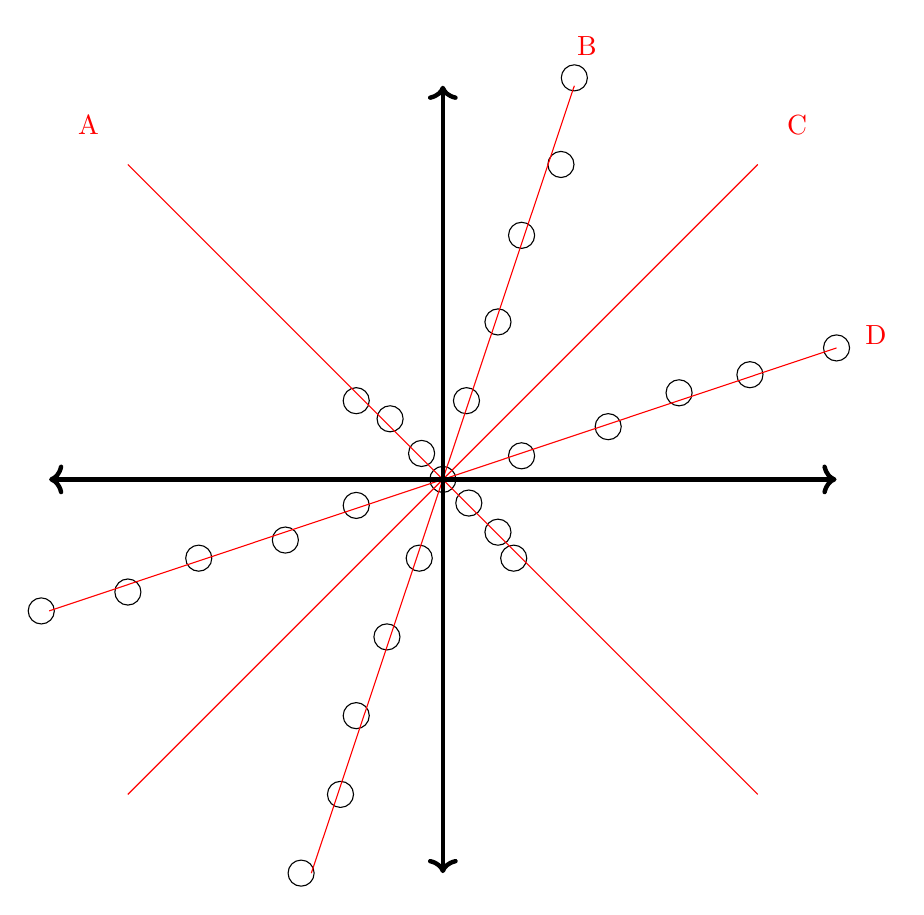
\begin{tikzpicture}
    \begin{scope}[every node/.style={circle,draw}]
    \node (O) at (0,0) {};
    \node (D2) at (1,0.30) {};
    \node (D3) at (2.1, 0.67) {};
    \node (D4) at (3,1.1) {};
    \node (D5) at (3.9,1.33) {};
    \node (D6) at (5,1.67) {};
    \node (D7) at (-1.1,-0.33) {};
    \node (D8) at (-2,-0.77) {};
    \node (D9) at (-3.1,-1.0) {};
    \node (D10) at (-4,-1.43) {};
    \node (D11) at (-5.1,-1.67) {};
    
    \node (B2) at (0.30,1) {};
    \node (B3) at (0.70,2) {};
    \node (B4) at (1.0,3.1) {};
    \node (B5) at (1.5,4) {};
    \node (B6) at (1.67,5.1) {};
    \node (B7) at (-0.30,-1) {};
    \node (B8) at (-0.71,-2) {};
    \node (B9) at (-1.1,-3) {};
    \node (B10) at (-1.30,-4) {};
    \node (B11) at (-1.80,-5) {};
    
    \node (A1) at (-.27, 0.33) {};
    \node (A2) at (-.67, 0.77) {};
    \node (A3) at (-1.1, 1.0) {};
    \node (A4) at (0.33, -0.30) {};
    \node (A5) at (0.70, -0.67) {};
    \node (A6) at (.90, -1.00) {};
    \end{scope}
    
    \draw[red] (-4, -4)--(4, 4);
    \draw[red] (-1.67, -5)--(1.67, 5);
    \draw[red] (-5, -1.67)--(5, 1.67);
    \draw[red] (-4, 4)--(4, -4);
    
    \node[red] (A) at (-4.5, 4.5) {A};
    \node[red] (C) at (4.5, 4.5) {C};
    \node[red] (B) at (1.83, 5.5) {B};
    \node[red] (D) at (5.5, 1.83) {D};

    
    \draw[<->,ultra thick] (-5,0)--(5,0);
    \draw[<->,ultra thick] (0, -5)--(0, 5); 
    \end{tikzpicture}
    \end{figure}
    \end{minipage}

    \part[2] \sall To get the principal components of the features, we calculate the eigenvectors of the covariance matrix, which are orthogonal, along with their corresponding eigenvalues. Which of the following are \textbf{consequences of the principal components being orthogonal to each other}?

    {\checkboxchar{$\Box$} \checkedchar{$\blacksquare$}
    \begin{checkboxes}
    % YOUR ANSWER
    % Change \choice to \CorrectChoice for the appropriate selection/selections
    \choice The variance of the data is maximized.
    \choice The reconstruction error is minimized.
    \CorrectChoice We can attribute certain variations in the data to unique principal components.
    \choice It ensures that our lower-dimensional data will be linearly separable.
    \choice None of the above
    \end{checkboxes}
    }
    

    \part[1] \sone If we wanted to perform dimensionality reduction to have just two features and train a classifier on them, we could represent our data by EITHER (a) picking any two features from the dataset, OR (b) using the first $2$ principal components we obtained from PCA. Which one should we prefer and why?

    {
    \begin{checkboxes}
    % YOUR ANSWER
    % Change \choice to \CorrectChoice for the appropriate selection/selections
    \choice We prefer (a), because it ensures randomness in the selection and have a better chance of representing the data well.
    \choice We prefer (a), because PCA introduces artificial bias and does not reflect the original features.
    \CorrectChoice We prefer (b), because PCA usually preserves higher variance than two original features.
    \choice We prefer (b), because PCA ensures that variance is evenly distributed across the features.
    \end{checkboxes}
    }
    

    \vspace{1cm}
    \fullwidth{\textbf{{\large PCA in Practice}}}
    
    \uplevel{
    For this section, refer to the PCA demo linked \href{https://colab.research.google.com/drive/17o9mWttvPnoWn8j9Upno8DfXrp2vlgUB}{here}. In this demonstration, we have performed PCA for you on a \href{https://en.wikipedia.org/wiki/Iris_flower_data_set}{simple four-feature dataset}. Run the code in the notebook, then answer the questions below based on the results. The questions have also been copied to the relevant code cells in the Colab notebook for ease.
    }
    
    \part[1] \sone Do you see any special relationships between any of the features? In particular, take a look at the \texttt{petal\_length} feature. How would you describe its association with each of the \textbf{other features}? Select the correct statement \textit{with appropriate justification.}

    \begin{checkboxes}
    % YOUR ANSWER
    % Change \choice to \CorrectChoice for the appropriate selection/selections
    \CorrectChoice The features are highly correlated: we observe linearly proportional relationships where increases in \verb|petal_length| often correspond to increases in another feature
    \choice The features are highly correlated: we observe that the color classes can be separated with decision boundaries along the \verb|petal_length| axis.
    \choice The features are uncorrelated: we observe random noise as if the features were generated from independent distributions
    \choice The features are uncorrelated: we observe the ``default $y=x$'' relationship between features
    \end{checkboxes}
        
    
    \part[1]  If we wanted to find $k$ principal components such that we preserve \textbf{at least} 95\% of the variance in the data, what would be the value of $k$? Hint: it is helpful here to look at the cumulative variance in the first $k$ components, which we have calculated for you.
    
    \begin{your_solution}[height=2cm, width=.15\textwidth, title=$k$]
    	2
    \end{your_solution}

    \clearpage


    \part[1]  See the visualization below of the first two principal components for the Fisher Iris Dataset (i.e. the projection of the Fisher Iris Dataset down to two dimensions), where the points are colored by label. From this graph, do you think PCA is an appropriate dimensionality reduction method for this dataset? Why or why not? Explain.

    \begin{figure}[H]
        \centering
        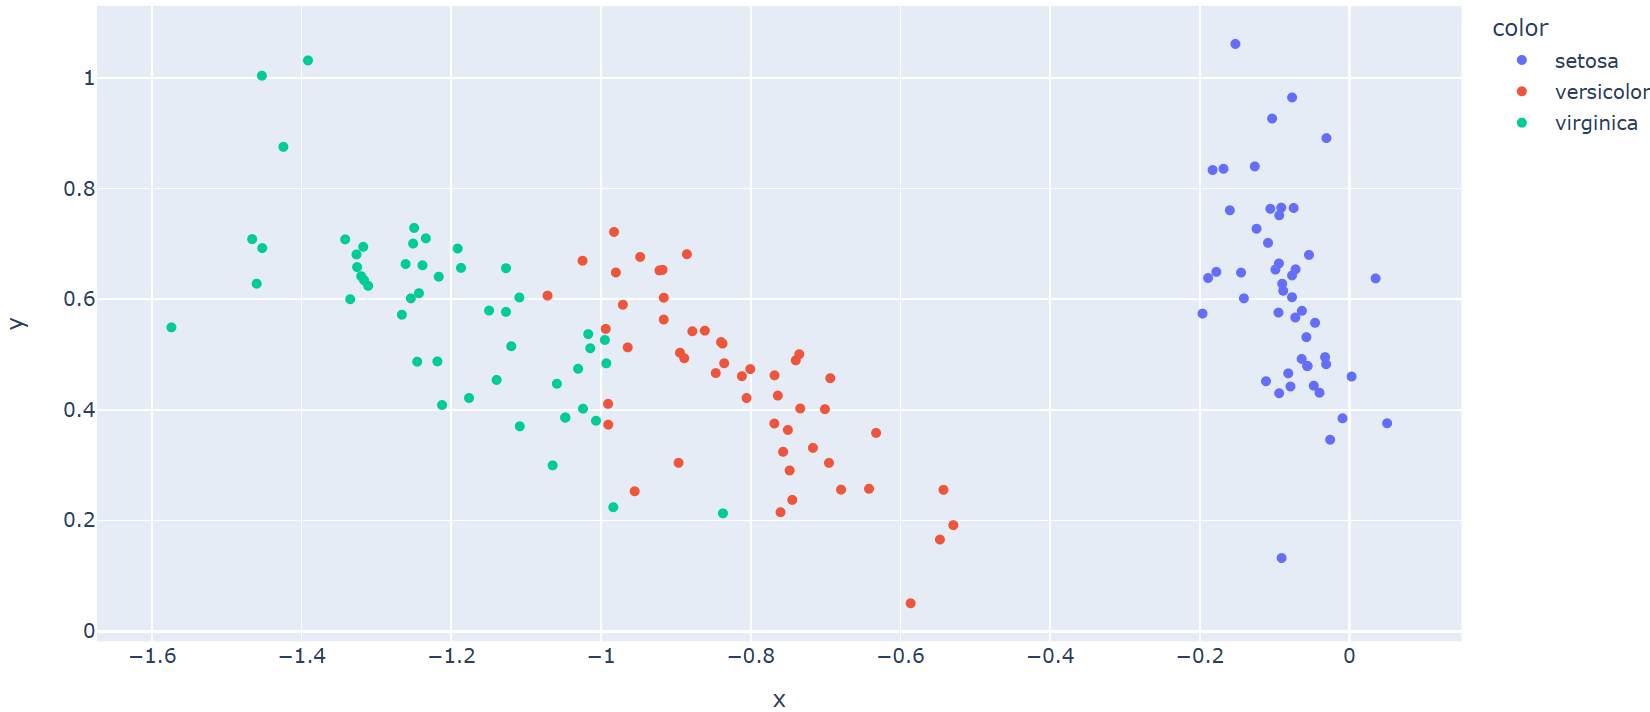
\includegraphics[width=0.95\linewidth, height=0.4\linewidth]{figures/2.7.png}
        \caption{Fisher Iris Dataset in 2D}
        \label{fig:KMeans2}
    \end{figure}
    
    \begin{your_solution}[title=Explanation, height=5cm, width=0.9\textwidth]
    	PCA is an appropriate dimensionality reduction method for the Fisher Iris Dataset as it preserves the variance and we can visualize the 2D data in Figure 1 that points are successfully clustered into its own kind of group. However, there are overlap between versicolor and virginica group of data points, meaning that PCA is not that good at separating low dimensional clusters away.
    \end{your_solution}
    
    


    
\end{parts}    \newpage
\sectionquestion{$k$-Means}
\label{sec:kmeans}

\begin{parts}
\part Consider the 2 datasets A and B. Each dataset is classified into $k$ clusters, with centers marked $X$ and cluster membership represented by different colors in the figure. For each dataset, exactly one clustering was generated by $k$-means with Euclidean distance. Select the image with clusters generated by $k$-means.

\begin{subparts}
\subpart[1] Dataset A

\begin{minipage}{.2\textwidth}
    \sone
    
    \begin{checkboxes}
    % YOUR ANSWER
    % Change \choice to \CorrectChoice for the appropriate selection/selections
    \CorrectChoice A.1
    \choice A.2
    \end{checkboxes}
\end{minipage}
\begin{minipage}{.75\textwidth}
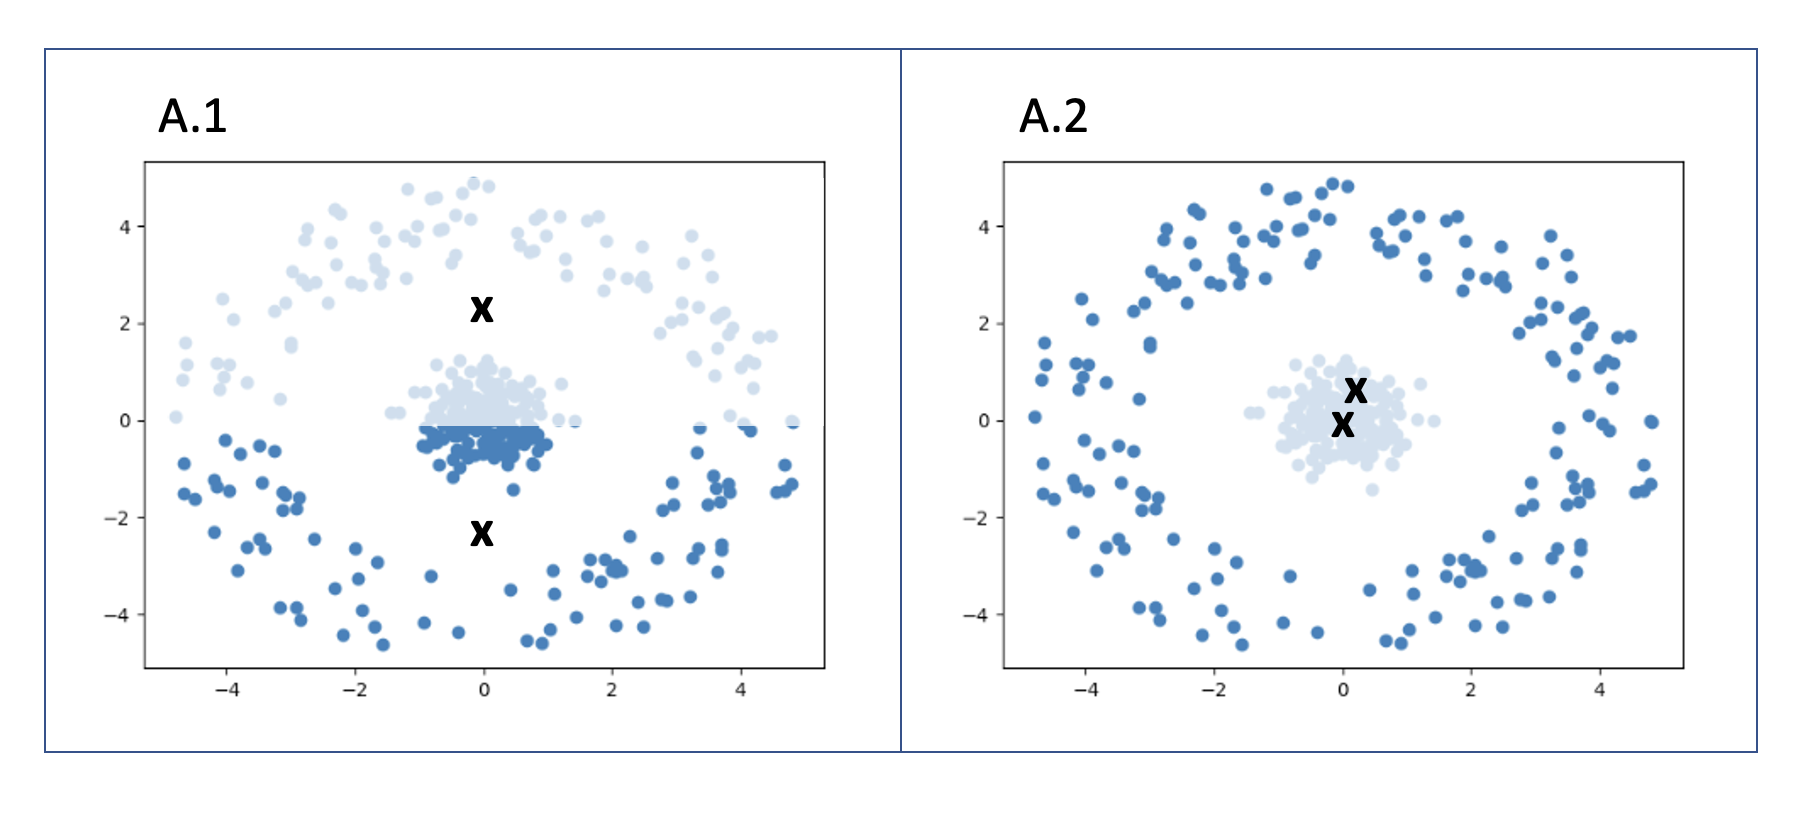
\includegraphics[width=.9\linewidth, height=5cm]{figures/4.1a.png}
\end{minipage}



\subpart[1] Dataset B

\begin{minipage}{.2\textwidth}
    \sone
    
    \begin{checkboxes}
    % YOUR ANSWER
    % Change \choice to \CorrectChoice for the appropriate selection/selections
    \CorrectChoice B.1
    \choice B.2
    \end{checkboxes}
\end{minipage}
\begin{minipage}{.75\textwidth}
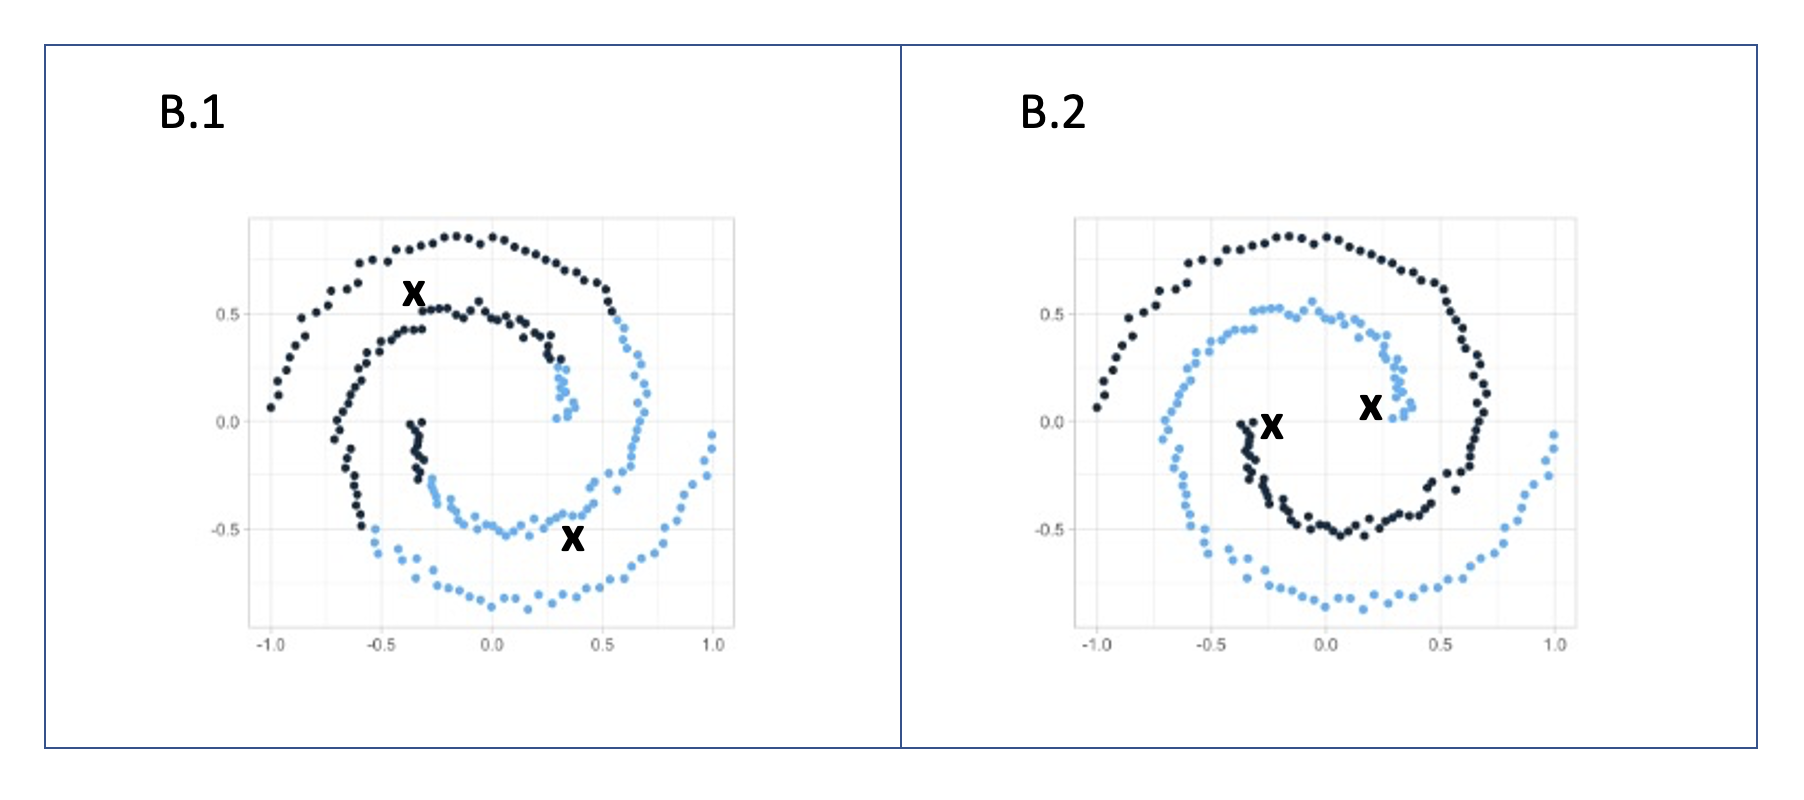
\includegraphics[width=.9\linewidth, height=5cm]{figures/4.1b.png}
\end{minipage}

\end{subparts}

\vspace{1em}
 \part Consider a dataset $\mathcal{D}$ with 5 points as shown below. Perform a $k$-means clustering on this dataset with $k=2$ using the Euclidean distance as the distance function.
 Remember that in the $k$-means algorithm, one iteration consists of following two steps: first, we assign each data point to its nearest cluster center; second, we recompute each center as the average of the data points assigned to it. Initially, the 2 cluster centers are chosen randomly as $\mu_0$ = (5.3, 3.5), $\mu_1$ = (5.1, 4.2). Parts (a) through (d) refer only to the first iteration of $k$-means clustering performed on $\mathcal{D}$.
 
\[
\mathcal{D}=\begin{bmatrix}
5.5&3.1\\
5.1&4.8\\
6.6&3.0\\
5.5&4.6\\
6.8&3.8\\
\end{bmatrix}
\]
    
    \clearpage 

    \begin{subparts}
    \subpart[1] \sone Which of the following points will be the new center for cluster 0?
    
    \begin{checkboxes}
    % YOUR ANSWER
    % Change \choice to \CorrectChoice for the appropriate selection/selections
    \choice (5.7 , 4.1)
    \choice (5.6 , 4.8)
    \CorrectChoice (6.3 , 3.3)
    \choice (6.7 , 3.4)
    \end{checkboxes}

    \subpart[1] \sone Which of the following points will be the new center for cluster 1?
    
    \begin{checkboxes}
    % YOUR ANSWER
    % Change \choice to \CorrectChoice for the appropriate selection/selections
    \choice (6.1 , 3.8)
    \choice (5.5 , 4.6)
    \choice (5.4 , 4.7)
    \CorrectChoice (5.3 , 4.7)
    \end{checkboxes}

    
    \subpart[1]  How many points will belong to cluster 0, using the new centers?
    
    
    \begin{your_solution}[title=Answer, height=2cm, width=3cm]
    	3
    \end{your_solution}


    
    % \subpart[1]  How many points will belong to cluster 1, using the new centers?
    
    
    % \begin{your_solution}[title=Answer, height=2cm, width=3cm]
    % \end{your_solution}
    


   \end{subparts}
   
   \vspace{1em}
   \part Recall that in $k$-means clustering we attempt to find $k$ cluster centers $\cv_1 ,\dots ,\cv_k$ such that the total distance between each point and the nearest cluster center is minimized. We thus solve
   $$ \argmin_{\cv_1 ,\dots ,\cv_k} \sum_{i=1}^N \min_{j\in\{1,\dots ,k\}} \|\xv^{(i)} - \cv_j\|_2^2 $$
   where $n$ is the number of data points. Instead of holding the number of clusters $k$ fixed, your friend John tries to also minimize the objective over $k$, solving 
   $$ \argmin_k \argmin_{\cv_1 ,\dots ,\cv_k} \sum_{i=1}^N \min_{j\in\{1,\dots ,k\}} \|\xv^{(i)} - \cv_j\|_2^2 $$

   You found this idea to be a bad one. 

    \begin{subparts}
    \subpart[1]  What is the minimum possible value of the objective function when minimizing over $k$? \\
    \begin{your_solution}[title=Answer, height=2cm, width=3cm]
    	N
    \end{your_solution}
    
    
    \subpart[1]  What is a value of $k$ for which we achieve the minimum possible value of the objective function when $N=100$? \\
    \begin{your_solution}[title=Answer, height=2cm, width=3cm]
    	100
    \end{your_solution}
    \end{subparts}
    
    \vspace{1em}
    \part  Consider the following brute-force algorithm for minimizing the $k$-means objective: Iterate through each possible assignment of the points to $k$ clusters, $\zv = [z^{(1)}, \ldots, z^{(N)}]$. For each assignment $\zv \in \{1,\ldots,k\}^N$, you evaluate the following objective function:
    $$J(\zv) = \argmin_{\cv_1, \ldots, \cv_k} \sum_{i=1}^N ||\xv^{(i)} - \cv_{z^{(i)}} ||_2^2$$
    At the end, you pick the assignment $\zv$ that had lowest $J(\zv)$.
    
    Suppose we have $N$ points and $k$ clusters. For how many possible assignments $\zv$ does the brute force algorithm have to evaluate $J(\zv)$?
    
   \begin{your_solution}[title=Answer, height=2cm, width=3cm]
   		$k^N$
    \end{your_solution}
    
   %  \begin{subparts}
   %  \subpart[1] Suppose we have $N$ points and $k$ clusters. For how many possible assignments $\zv$ does the brute force algorithm have to evaluate $J(\zv)$?
    
   % \begin{your_solution}[title=Answer, height=2cm, width=3cm]
   %  \end{your_solution}


   %  \subpart[1] Suppose $N=1000$, $k=10$, and it takes us $0.01$ seconds to evaluate $J(\zv)$ for a single assignment $\zv$. How many seconds will the brute force algorithm take to check all assignments?
    
   % \begin{your_solution}[title=Answer, height=2cm, width=3cm]
   %  \end{your_solution}
   %  \end{subparts}
    
    \vspace{1em}
    \part Initializing the centers has a big impact on the performance of the $k$-means clustering algorithm. Usually, we randomly initialize $k$ cluster centers. However, there are other methods, namely, furthest point initialization and $k$-means++ initialization.
    
    \begin{subparts}
    \subpart[1] \sone
     Clustering at convergence generated by furthest point initialization is sensitive to outliers. Which of the following statements is correct about this phenomenon?
    
    \begin{checkboxes}
    % YOUR ANSWER
    % Change \choice to \CorrectChoice for the appropriate selection/selections
    \choice Although outliers will not be selected in the first several iterations, they will temporarily be chosen as centers during training.
    \choice Outliers will slow convergence, but will never be centers at convergence time.
    \CorrectChoice Outliers are likely to be selected as centers in the first few iterations.
    \end{checkboxes}
    \clearpage
    \begin{figure}[H]
        \centering
        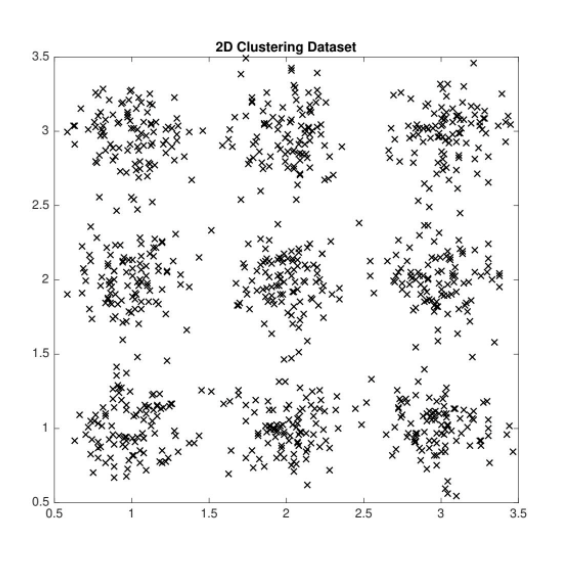
\includegraphics[width=0.5\linewidth, height=0.5\linewidth]{figures/kmeans.png}
        \caption{2D Dataset}
        \label{fig:KMeans2}
    \end{figure}
    
    
    \subpart[1] 

    \sone Using the dataset in Figure \ref{fig:KMeans2} above, compared to random initialization, using $k$-means++ initialization is \rule{1cm}{0.01mm}.

    
    \begin{checkboxes}
    % YOUR ANSWER
    % Change \choice to \CorrectChoice for the appropriate selection/selections
    \CorrectChoice more likely to choose one sample from each cluster because centers are chosen with probability proportional to squared distance from existing centers.
    \choice less likely to choose one sample from each cluster because the formula does not account for the number of clusters which may be found and thus won't be calibrated to correctly choose one point from each cluster.
    \choice equally likely to choose one sample from each cluster because as the number of points grows large, $k$-means++ asymptotically approaches random initialization.
    
    \end{checkboxes}


    \end{subparts}

\end{parts}
    \newpage
\sectionquestion{Ensemble Methods}
\label{sec:ensemble}

\begin{parts}
\part[1] \tf In a random forest, it is generally better for the trees to be highly correlated, as this reduces ensemble variance.
\begin{checkboxes}
\choice True
\CorrectChoice False
\end{checkboxes}

\part[2] \sall Which of the following is true about OOB error?

{\checkboxchar{$\Box$} \checkedchar{$\blacksquare$}
\begin{checkboxes}
\choice OOB error is calculated on a held-out dataset separate from the dataset used to generate bootstrap samples
\CorrectChoice OOB error is the aggregated value of the errors of subsets of the ensemble on samples those subsets were not trained on 
\choice Cross-validation error is the same as OOB error
\CorrectChoice OOB error can be used instead of validation error when hyperparameter tuning a random forest model
\choice None of the above
\end{checkboxes}}


\part[2] \sall Which of the following are hyperparameters that can be tuned in a random forest?

{\checkboxchar{$\Box$} \checkedchar{$\blacksquare$}
\begin{checkboxes}
\CorrectChoice Number of trees trained
\CorrectChoice Number of points used to train each decision tree
\CorrectChoice Size of feature subsets used to train each decision tree
\choice Which features are used for splits in each decision tree 
\choice None of the above
\end{checkboxes}}



\part In this question, we will consider the behavior of an error bound for random forests in the case of \textbf{binary classification}. Given a random forest of $B$ trees $\{ h_i(x) \}_{i=1}^B$ and a sample $(x,y)$ drawn from some data distribution $\mathcal{D}$, define the classification margin as:
\[
m(x, y) = \frac{1}{B} \left(\sum_{i=1}^B \Ib[h_i(x) = y] -  \sum_{i=1}^B \Ib[h_i(x) \neq y] \right)
\]
In words, the margin $m(x,y)$ is the difference between the average vote for the correct label and the average vote for the incorrect label.

\begin{subparts}
\subpart[1] \textbf{Fill in the blank:} For any example $(x,y)$, the example is classified incorrectly if and only if $m(x,y) \leq \underline{\qquad}$. Assume majority vote ties are classified incorrectly.

\begin{your_solution}[title=Answer,height=2cm, width=3cm]
    %solution
    0
\end{your_solution}


\subpart[1] \sone Using \href{https://en.wikipedia.org/wiki/Chebyshev%27s_inequality}{Chebyshev's inequality}, it is possible to bound the generalization error of a random forest as $P(m(x,y) < c) \leq \frac{\text{Var}(m(x,y))}{s^2}$, where $c$ is your answer to part (a) and $s$ is the \emph{strength} of the ensemble $$s = \mathbb{E}_{(x,y) \sim \mathcal{D}}[m(x,y)].$$ 

Through some additional manipulation, it is further possible to show that ${\text{Var}(m(x,y)) \leq \overline{\rho}(1 - s^2)}$, where $\overline{\rho}$ is the mean correlation between trees in the ensemble. Substitute this into the given bound. Which of the following describes how the error bound is affected by $s$ and $\overline{\rho}$?

\begin{checkboxes}
    % YOUR ANSWER
    % Change \choice to \CorrectChoice for the appropriate selection/selections
    \choice The error bound gets smaller as $\overline{\rho}$ increases and $s$ increases.
    \choice The error bound gets smaller as $\overline{\rho}$ increases and $s$ decreases.
    \CorrectChoice The error bound gets smaller as $\overline{\rho}$ decreases and $s$ increases.
    \choice The error bound gets smaller as $\overline{\rho}$ decreases and $s$ decreases.
    \end{checkboxes}
\end{subparts}

\clearpage

\part[1]  \tf Consider some training point $(x^{(i)}, y^{(i)})$ to the AdaBoost algorithm. If for all $t$, the weak learner $h_t$ learned during training at time $t$ correctly classifies $h_t(x^{(i)}) = y^{(i)}$, there will eventually be a finite time $t$ such that the weight assigned to $x^{(i)}$ in the training distribution $\D_t$ reaches exactly $0$.

    \begin{checkboxes}
    % YOUR ANSWER
    % Change \choice to \CorrectChoice for the appropriate selection/selections
    \choice True
    \CorrectChoice False
    \end{checkboxes}


\part Assume we use a deterministic training procedure for weak learners. Suppose for some iteration $t'$ of AdaBoost we find that the weak classifier learned by the algorithm at time $t'$ has error $\epsilon_{t'} = 0.5$ of the weak learner $h_{t'}$ on the training distribution weighted by $\mathcal{D}_{t'}$.

\begin{subparts}
\subpart[1]What weight $\alpha_{t'}$ will AdaBoost assign to the classifier $h_{t'}$ from above?

    
\begin{your_solution}[title=$\alpha_{t'}$,height=2cm, width=3cm]
    %solution
    0
\end{your_solution}

\subpart[1] \textbf{Select all that apply:} In which of the following cases will $\mathcal{D}_{t' + 1} (i) > \mathcal{D}_{t'} (i)$ (in other words, in which of the following cases will the weight of training sample $(x^{(i)}, y^{(i)})$ \textit{strictly} increase from time step $t'$ to $t'+1$)?
    {%
    \checkboxchar{$\Box$} \checkedchar{$\blacksquare$} % change checkbox style locally
    \begin{checkboxes}
     \choice $h_{t'} (x^{(i)}) = y^{(i)}$ ($h_{t'}$ classifies $x^{(i)}$ correctly)
     \choice $h_{t'} (x^{(i)}) \neq y^{(i)}$ ($h_{t'}$ classifies $x^{(i)}$ incorrectly)
     \CorrectChoice None of the above.
    \end{checkboxes}
    }

\subpart[1] \sall Which of the following are true about the next iteration of the AdaBoost algorithm?
{\checkboxchar{$\Box$} \checkedchar{$\blacksquare$}
\begin{checkboxes}
\CorrectChoice The errors $\epsilon_{t'+1}$ and $\epsilon_{t'}$ are equivalent
\CorrectChoice The weak learners $h_{t'+1}$ and $h_{t'}$ will be equivalent (i.e., they will have the same output for every input)
\choice None of the above
\end{checkboxes}}


\end{subparts}

\end{parts}

\newpage    \newpage
\sectionquestion{Recommender Systems}
\label{sec:recsys}

\begin{parts}

 \part[2] \sall In which of the following situations will a collaborative filtering system be a more appropriate learning algorithm than a linear or logistic regression model?
    
    
    {\checkboxchar{$\Box$} \checkedchar{$\blacksquare$}
        \begin{checkboxes}
        % YOUR ANSWER
        % Change \choice to \CorrectChoice for the appropriate selection/selections 
        \CorrectChoice You manage an online bookstore, and you have book ratings and sales data from many users. For each user, you want to recommend other books she will enjoy, based on her own ratings and the ratings of other users.
        \choice You manage an online bookstore, and you have book ratings and sales data from many users. You want to learn to predict the expected sales volume (number of books sold) as a function of the average rating of a book.
        \CorrectChoice You run an online news aggregator, and for every user, you know some subset of articles that the user likes and some different subset that the user dislikes. You want to use this to find other articles that a given user likes.
        \choice You've written a piece of software that downloads news articles from many news websites. In your system, you also keep track of which articles you personally like and which ones you dislike, and the system also stores away features of these articles (e.g., word counts, name of author). Using this information, you want to build a system to try to find additional new articles that you personally will like.
        \choice None of the above
        \end{checkboxes}
    }

 

 \part[2] \sall What is the basic intuition behind matrix factorization?
    
    
    {\checkboxchar{$\Box$} \checkedchar{$\blacksquare$}
        \begin{checkboxes}
        % YOUR ANSWER
        % Change \choice to \CorrectChoice for the appropriate selection/selections 
        \choice That content filtering and collaborative filtering are just two different factorizations of the same rating matrix.
        \choice That factoring user and item matrices can partition the users and items into clusters that can be treated identically, which can reduce computation when making recommendations by retaining only representative users or items in each cluster.
        \choice That computing a user-user or item-item correlation is more efficient when first factoring matrices, even when including the cost of factoring matrices.
        \CorrectChoice That users and items can be well described in a shared low dimensional space that can be computed from the rating matrices.
        \choice None of the above
        \end{checkboxes}
    }
    
    
    
\part Neural the Narwhal decides to set up a friend-recommendation system for all the students in 10-301/601, of which there are $N = 10,301,601$. Ideally, Neural would store the full $N \times N$ matrix $M$, where $M_{ij}$ is 1 if student $i$ and $j$ are friends, 1 if $i = j$, 0 if student $i$ and $j$ are nemeses, or \texttt{null} if students $i$ and $j$ have never met. Assume that these are the only possible relationships between 2 people and that all relationships are symmetric (so it cannot be the case that student $i$ thinks student $j$ is their friend while $j$ thinks $i$ is their nemesis). Unfortunately, storing $M$ in its entirety would take over 10 TB of storage, which Neural cannot afford on a TA salary. Neural instead uses the following procedure to approximate $M$ as $U U^T$ for some low rank $N \times d$ matrix $U$, where each row of $U$ corresponds to a student.

\algrenewcommand{\algorithmiccomment}[1]{\hfill// #1}
\algtext*{EndWhile}% Remove "end while" text
\algtext*{EndIf}% Remove "end if" text
\begin{algorithm}
\begin{algorithmic}[1]
\State Given learning rate $\eta$, ground truth relationships $M$
\State Randomly initialize user embedding matrix $U \in \mathbb{R}^{N \times d}$

\While{not converged}
    \State Sample $i \sim$ Uniform(1, $N$), $j \sim$ Uniform(1, $N$)
    \State $\hat{M}_{ij} \gets \sigma(\vec{u}_i^T \vec{u}_j)$ 
    \Comment{$\sigma$ is sigmoid function}
    \State $\mathcal{L}(\vec{u}_i, \vec{u}_j) \gets -M_{ij} \log(\hat{M}_{ij}) - (1-M_{ij})\log(1 - \hat{M}_{ij})$
    \Comment{Compute logistic loss}
    \State $\vec{g}_i \gets \nabla_{\vec{u}_i} \mathcal{L}(\vec{u}_i, \vec{u}_j)$
    \Comment{Compute and perform gradient updates}
    \State $\vec{g}_j \gets \nabla_{\vec{u}_j} \mathcal{L}(\vec{u}_i, \vec{u}_j)$
    \State $\vec{u}_i$ $\gets$ $\vec{u}_i$ - $\eta \cdot \vec{g}_i$
    \State $\vec{u}_j$ $\gets$ $\vec{u}_j$ - $\eta \cdot \vec{g}_j$
\EndWhile
\end{algorithmic}
\end{algorithm}
\newpage
\begin{subparts}
\subpart[1] Explain why line 4 of the algorithm is incorrect.
You do not need to provide a line of code unless you feel that it would help you in your explanation.

    \begin{your_solution}[title=Explanation, height=3cm, width=0.9\textwidth]
    	The line 4 does not account for the symmetry property of the relationship matrix $\hat{M}$, meaning that the updates for $u_i$ and $u_j$ that updates $\hat{M_{ij}}$ in an iteration may not be necessarily identical to the updates for $u_j$ and $u_i$ that updates $\hat{M_{ji}}$ later. It would violates the symmetric relationship describing in the problem: all relationships are symmetric.
    \end{your_solution}

\subpart[1] \sone Based on the loss function given on line 6, derive an expression for $\nabla_{\vec{u}_j} \mathcal{L}(\vec{u}_i, \vec{u}_j)$ in terms of $\vec{u}_i$, $\vec{u}_j$, and $M_{ij}$. Note that $\sigma$ denotes the sigmoid function and $\log$ is natural log.
    %
    \begin{checkboxes}
    % YOUR ANSWER
    % Change \choice to \CorrectChoice for the appropriate selection/selections
    \choice $\vec{u}_i M_{ij} \sigma(\vec{u}_i^T \vec{u}_j)$
    \choice $\vec{u}_i(M_{ij} + \sigma(\vec{u}_i^T \vec{u}_j))$
    \CorrectChoice $\vec{u}_i(-M_{ij} + \sigma(\vec{u}_i^T \vec{u}_j))$
    \choice None of the above.
    \end{checkboxes}
         
    

\subpart[2] \sall Why is it appropriate here to factorize $M$ as the product of a single matrix by itself $U U^T$ rather than as the product of two distinct matrices $VW^T$?
    {\checkboxchar{$\Box$} \checkedchar{$\blacksquare$}
    \begin{checkboxes}
    % YOUR ANSWER
    % Change \choice to \CorrectChoice for the appropriate selection/selections
    \CorrectChoice $U U^T$ enforces that our approximation is symmetric, while $VW^T$ is not necessarily symmetric.
    \choice SGD is guaranteed to converge faster and to a better optimum for $U$ because we have fewer parameters to learn.
    \choice We can parallelize training for $U$, whereas we could not parallelize training for $V$ and $W$.
    \CorrectChoice We wish to model relationships between objects of a single type, not between objects of two different types.
    \choice None of the above.
    \end{checkboxes}
    }
    

\end{subparts}

\end{parts}
    \newpage
\newpage
\section{Collaboration Questions}
After you have completed all other components of this assignment, report your answers to these questions regarding the collaboration policy. Details of the policy can be found \href{http://www.cs.cmu.edu/~mgormley/courses/10601/syllabus.html}{here}.
\begin{enumerate}
    \item Did you receive any help whatsoever from anyone in solving this assignment? If so, include full details.
    \item Did you give any help whatsoever to anyone in solving this assignment? If so, include full details.
    \item Did you find or come across code that implements any part of this assignment? If so, include full details.
\end{enumerate}

\begin{your_solution}[height=6cm]
% YOUR ANSWER 
\begin{enumerate}
	\item No.
	\item No.
	\item No.
\end{enumerate}
\end{your_solution}
    \newpage
    \end{questions}
\end{document}